\chapter{Entwicklungsstartegie}
\label{chap:git-strat}

Das Projekt wird auf mehreren Branches entwickelt, damit eine saubere Trennung zwischen Entwickung und produktivem Code gewährleistet ist. Dazu wird auf die GitFlow branching Strategie gesetzt\cite{Atlassian2024}. 

Hierbei gibt es zwei Hauptbranches: Zum einen den \glqq main\grqq-Branch, der den produktiven Code enthält und dessen Build-Artifakte in die prokutive Umgebung deployt werden und den \glqq develop\grqq-Branch auf dem die aktive Entwicklung stattfindet. 

Einzelne Features werden auf sogennanten Feature-Branches entwickelt. Ist ein Feature fertig entwickelt, kann es auf dem \glqq develop\grqq-Branch integriert werden. Auf dem \glqq develop \grqq-Branch können dann auch umfassendere Tests laufen, die sicher stellen, dass das der Merge des Feature-Branches nicht zu einer Destabilisierung des gesammt Systems geführt hat. Wenn der \glqq develop\grqq-Branch alle Tests duchlaufen hat und alle Features die für den nächsten Release gewünscht waren fertig entwickelt sind, wird der \glqq develop\grqq in den \glqq main\grqq-Branch gemergt, was zu einem neuen Release führt.

Zusätzlich gibt es für schnelle Paches von wichtigen Fehlern die Möglichkeit \glqq hotfix\grqq-Branches anzulegen, die direkt in den \glqq main\grqq-Branch gemergt werden dürfen.

Wenn mehrere Entwickler an einem Projekt, das eine solche Branching-Strategie verfolgt, arbeiten, dann sollten Branch-Protection-Rules eingesetzt werden um die beiden Hauptbranches zu schützen. So bietet es sich z.B. an dass für einen Merge auf \glqq develop\grqq{} oder \glqq main\grqq{} immer ein Reviewer einen den Pull-Request genehmigen muss. Außderdem kann es sinnvoll sein, dass bestimmte Tests nicht ausfallen dürfen bevor auf den \glqq develop\grqq{} oder \glqq main\grqq{} branch gemerged wird.

Bei der Bennenung der Branches sollte der Typ als Präfix vorangestellt werden. So könnte ein Feature-Branch z.B. \lstinline{feature/eigenvektor-finder} und ein bugfix branch \lstinline{bugfix/inverted-matrix-multiplication} heißen.

\begin{figure}
    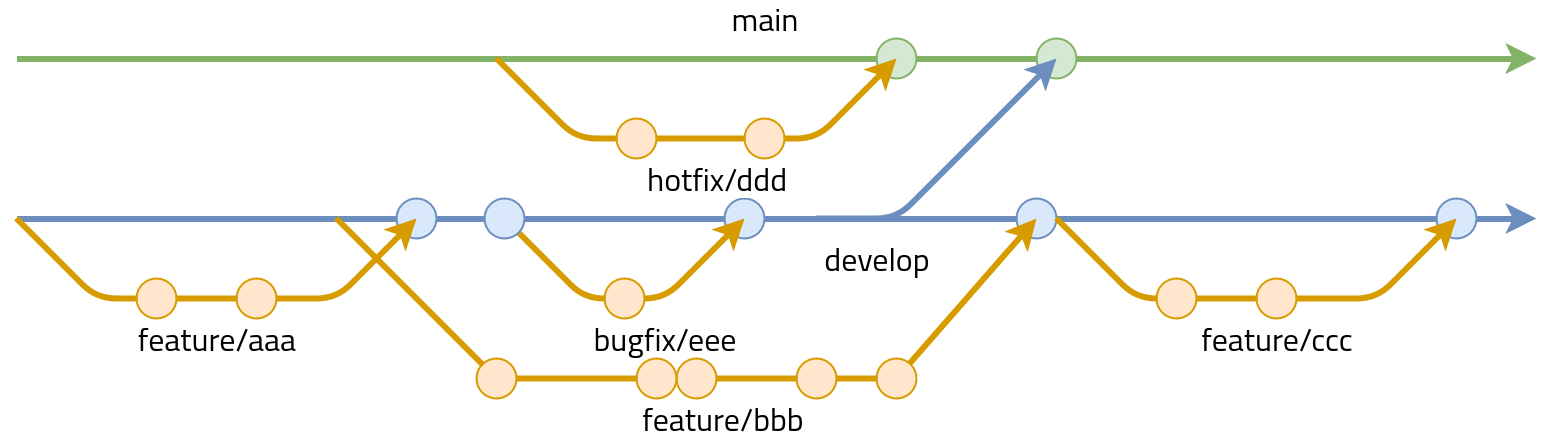
\includegraphics[scale=0.25]{res/branching_scheme.drawio.png}
    \caption{Vereinfachte Darstellung eines Branch-Graphs bei Anwendung des beschriebenen Branching Schemas.}
\end{figure}
